\documentclass[]{spie}  %>>> use for US letter paper
%%\documentclass[a4paper]{spie}  %>>> use this instead for A4 paper
%%\documentclass[nocompress]{spie}  %>>> to avoid compression of citations
%% \addtolength{\voffset}{9mm}   %>>> moves text field down
%% \renewcommand{\baselinestretch}{1.65}   %>>> 1.65 for double spacing, 1.25 for 1.5 spacing 
%  The following command loads a graphics package to include images 
%  in the document. It may be necessary to specify a DVI driver option,
%  e.g., [dvips], but that may be inappropriate for some LaTeX 
%  installations. 
\usepackage[]{graphicx}
\usepackage{subfigure}
\usepackage{amsmath}


\graphicspath{{images/}}

\title{CIVILITY: Cloud based Interactive Visualization of Tractography Brain Connectome} 

\author{Dana\"{e}le Puechmaille\supit{a}, Juan C. Prieto\supit{a} and Martin Styner\supit{a}
\skiplinehalf
\supit{a}Neuro Imaging Reasearch and Analysis Laboratory, Department of Psychiatry, \\
 University of North Carolina, Chapel Hill, North Carolina, United States;
}

%>>>> Further information about the authors, other than their 
%  institution and addresses, should be included as a footnote, 
%  which is facilitated by the \authorinfo{} command.

\authorinfo{Further author information: (Send correspondence to J.C.P)\\J.C.P.: E-mail: jprieto@med.unc.edu\\D.P: E-mail:danaele@email.unc.edu\\M.S.: styner@cs.unc.edu}
%%>>>> when using amstex, you need to use @@ instead of @
 

%%%%%%%%%%%%%%%%%%%%%%%%%%%%%%%%%%%%%%%%%%%%%%%%%%%%%%%%%%%%% 
%>>>> uncomment following for page numbers
 \pagestyle{plain}    
%>>>> uncomment following to start page numbering at 301 
%\setcounter{page}{301} 
 
  \begin{document} 
  \maketitle 

%%%%%%%%%%%%%%%%%%%%%%%%%%%%%%%%%%%%%%%%%%%%%%%%%%%%%%%%%%%%% 
\begin{abstract}

We propose a new tool named Cloud based Interactive Visualization of Tractography Brain Connectome (CIVILITY) which is an interactive visualization tool of brain connectome in the web.
CIVILITY is a web application and has mainly 2 components.

- CIVILITY-visualization ; front end of the application. This is a circular plot of the brain connectivity using the method of visualization : Hierarchical Edge Bundling. The graphic visualization of the brain connectivity is generated using Data Driven Documents (D3.js) \footnote{https://github.com/d3/d3}.

- CIVILITY-tractography ; analysis pipeline. The analysis of the brain connectome is computed using a probabilistic tractography method (FSL tools : bedpostx and probtrackx2) using surfaces as seeds. Seeds surfaces are created with the ExtractLabelSurfaces\footnote{https://github.com/NIRALUser/ExtractLabelSurfaces}.

CIVILITY performs the brain connectivity analysis in remote computing grids where the CIVILITY-tractography pipeline is deployed. CIVILITY uses clusterpost\footnote{https://github.com/NIRALUser/clusterpost} to submit the jobs to the computing grid. 
%Clusterpost is a server application providing a REST api to submit jobs in remote computing grids using. Data transfer, job execution and monitoring are all handled by clusterpost.
The front end of CIVILITY submits tasks to clusterpost and retrieves results when they are finished.
This work is motivated by medical applications in which brain connectivities need to be computed automatically and analyzed easily.

This paper is submitted to the SPIE Medical Imaging 2016 conference in the category Image processing. 

\end{abstract}

%>>>> Include a list of keywords after the abstract 

\keywords{Tractography, connectivity, diffusion tensor imaging, atlas, visualization, brain connectome, open source software, cloud}

%%%%%%%%%%%%%%%%%%%%%%%%%%%%%%%%%%%%%%%%%%%%%%%%%%%%%%%%%%%%%
\section{INTRODUCTION}
\label{sec:intro}

Tractography has found many applications over the past decade. Some applications include neurosurgical planning; assessment and study of neurological diseases such as multiple sclerosis  or schizophrenia; and post-surgical validation. However the analyze of the connectivity matrix is not intuitive and easy to interpret. That's why this application offers to researchers an interactive web interface to show the connectivity clearly according to some parameters. 

In this paper, we present CIVILITY an open source web application hosted in a cloud. This tool offers to researchers the possibility to launch a unique tractography script and to visualize the brain connectome interactively. Each user is identified by a user account associated with privileges and can access to his results from anywhere in the cloud.
The tractography pipeline uses the probabilistic method  of tractography\footnote{describe all possible trajectories} using surfaces as seeds (FSL tools : bedpostx and probtrackx). The tractography pipeline is executed on the computing grid and once is finished results are retrieved and brain connectome visualization is available. 
The graphic visualization of the brain connectome is generated using Data Driven Documents (D3.js) and more precisely the method Hierarchical Edge Bundling. This is a circle plotting representing the brain connectivity. All links can be threshold between two values, their shape can also be modified for an easier visualization. This tool is submitted at the SPIE Medical Imaging 2016 conference in the category Image processing and we seek to enable further clinical and research applications of tractography.

In summary, CIVILITY performs tractography by sending jobs in remote computing grid using the tool clusterpost. Once the tractography is finished, the results are retrieved and the brain connectome is visualized interactively. Results and visualization are accessible from any system in the cloud.
In order to validate this pipeline, we applied the tractography pipeline to a dataset and retrieves results for analyzing the brain connectome through the visualization tool.

The following section explains in detail the methods used in CIVILITY.

\section{METHODS} 
\label{sec:METHODS}

This section explains in details the two components of CIVILITY : tractography and visualization.
The figure \ref{fig:architectureCIVILITY} shows the architecture of the application CIVILITY. 

\begin{figure}
\centering 
\subfigure[]{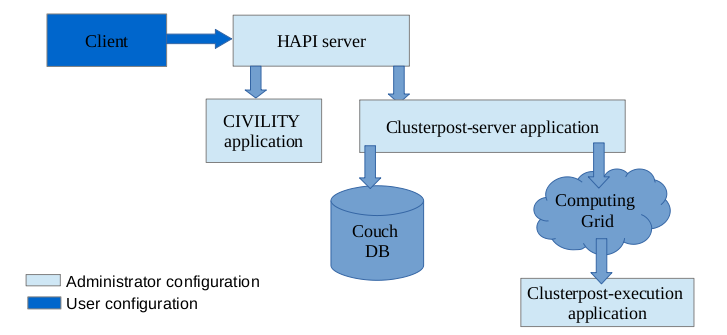
\includegraphics[width=15cm]{architectureCIVILITY.png}}
\caption[Architecture of the application CIVILITY]{Architecture of the application CIVILITY}
\label{fig:architectureCIVILITY}
\end{figure} 

\subsection{Tractography}

The tractography is the computation of the brain connectivity. First, the form to complete for launch a tractography job will be described. Then, the tractography pipeline explains in details.

\subsubsection{Tractography form}

First, a tractography form is used to upload data and set tractography parameters.
All data required for the tractography must be already been registered in the same space : DWI space (or Diffusion space). The images to provide are : Diffusion weighted imaging (DWI), T1 reference image, brain mask and must be in the NRRD format. The tractography pipeline uses the probabilistic method of tractography using surfaces as seeds. Thus a brain surface representing the white matter must be uploaded. The surface to provide must be a VTK file and must contain label information ( and must be also in DWI space). If there isn't label information, another VTK surface, with the same mesh and containing labels, must be uploaded. The name of the labelset in the VTK file must be known and specified in the tractography form. All labels are identified by an ID, it is possible to ignore a ROI in the tractography by setting the label ID in the form. 
In addition, a JSON file must be upload. This file describe the parcellation table: seeds names, labels id, matrix order, etc.). 
As explained before, the tratography uses FSL tools : bedpostx and probtrackx. The number of tensors in the voxel fitting is set to 2 by default, but can be modified by the user.

\subsubsection{Tractography pipeline}

In this section the pipeline is described. 

First, The tool DWIConvert\footnote{https://github.com/BRAINSia/BRAINSTools/tree/master/DWIConvert} is used to convert nrrd to nifti images, this last format is required to use FSL tools in tractography.
Then, bedpostx tool is used to build default distributions of diffusion parameters at each voxel(2 tensors in the voxel fitting).
This method of tractography is using surfaces as seeds. These surfaces  (ASCII format) are created with the C++ tool : ExtractLabelSurfaces apply on the White Matter surface (VTK file) containing labels.
Probtrackx2 is the probabilistic tractography, it runs on the output of bedpostX and according to a seed list. The seed list is created according to the atlas describe in the json file. Each seed is a surface.  The label extraction can used overlapping or not between each ROIs. The tractography result is a connectivity matrix.
Once the tractography done, CIVILITY allow users to visualize easily the connectivity matrix like explained in the following section. 

The entire pipeline is available in the github project repository\footnote{https://github.com/NIRALUser/CIVILITY} or in the NITRC page\footnote{https://www.nitrc.org/projects/civility/}.

\subsection{Visualization}

CIVILITY-visualization is the front end of the application. The brain connectome can be visualized using results from the tractography computed in the computing grind. 
Tractography results are shown in a summary jobs table. For each job, the job status is printed and when a job is done, an interactive plotting is available. The interactive visualization is also usable by uploading files from user system. The files required are : the connectivity matrix (output of probtrackx2 : fdt\_network\_matrix) and the parcellation table description (JSON file).

\subsubsection{Matrix Computation}

The matrix is first normalized by the number of fibers per rows. The circle plot shows a triangular matrix computed by the maximum, minimum or average between upper and lower triangular matrices according to the user selection in the web interface. 
Finally, each value in the triangular matrix represents the connectivity value between 2 ROIs. The connectivity value is represented in percentage, the value is a pourcentage of probability that streamlines from a specific seed go to another one.

\subsubsection{Visualization parameters}

The brain connectome is plotting as circle plot, generated using Data Driven Documents (D3.js) and more precisely the method Hierarchical Edge Bundling. Another, connectivity visualization is available : brain connectivity on brain templates\footnote{https://www.nitrc.org/projects/bnv}.
As explained before, the user selects the way how to compute the triangular matrix : average, maximum or minimum between lower and upper triangles of the matrix. 
A tension value can be set to change the shape of the links, also the diameter of the circle is adjustable.
For an easier visualization, the connectivity visualized is threshold between 2 values set : the maximum upper value and the threshold value. Users can change these values to print the brain connectome as precisely as they want. The links under the threshold value are not print and links above the maximum upper value are print in red. 
Links colors  indicate the connectivity value according to the colorbar corresponding. The thickness of links is proportional to the connectivity value.

The following section describes the materials used in CIVILITY.

\section{MATERIALS}

We apply our tractography pipeline to 19 infants (scanned at 1 year and 2 years approximately).
All data had previously been Quality Control (QC) and registered in the same space : DWI space. The surface contains labels information according to the brain atlas AAL90. 
The following section shows the results of this pipeline. 

\section{RESULTS} 

We compute the brain connectome of these 19 infants at two ages : 1 year and 2 years. The tractography computed with FSL tools is using 2 tensors in the voxel fitting. The method of computation we have chosen is using surfaces as seeds. Each surface corresponds to a brain region in the atlas Automated Anatomical Labeling (AAL). All ROIs surfaces overlap with each others. The cerebellum regions are ignored in the brain connectome computation. The number of samples is set to 3000 (number of streamlines per voxel) with a step length of 0.75mm and a seed sphere sampling of 0.5. 

The first observation we can do is : an higher time of computation for 2 year old subjects compare to 1 year old subjects. This time difference is explained by the size of the brain of the infant, more the brain is big, more the time of computation is high.

We make some statistics on this dataset presented in the next section.

\subsection{Brain connectome average}

We compute on our dataset the average brain connectome at each year : 1 and 2 years. 

\begin{equation}
	A_{i,j} = \frac{\sum_{i=0}^n M_i}{n}
	\label{equ:average}
\end{equation}

Equation \ref{equ:average} defines the average brain connectome for n connectivity matrices M$_{i}$. 

We threshold the plotting between : 0.01 and 0.4 for a better visualization.
The connectivity visualized is computed with the average value between the lower and upper triangles of the connectivity matrix.

\begin{figure}
\centering 
\subfigure[]{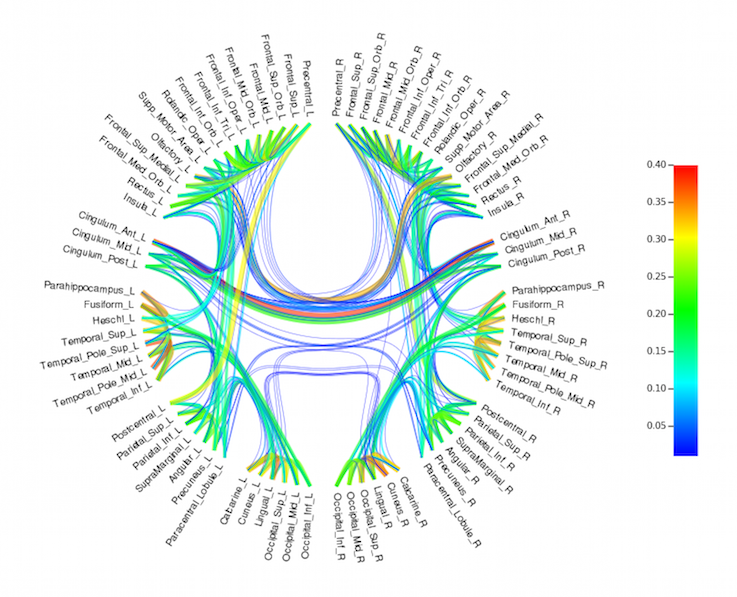
\includegraphics[width=8cm]{average_1y.png}}
\subfigure[]{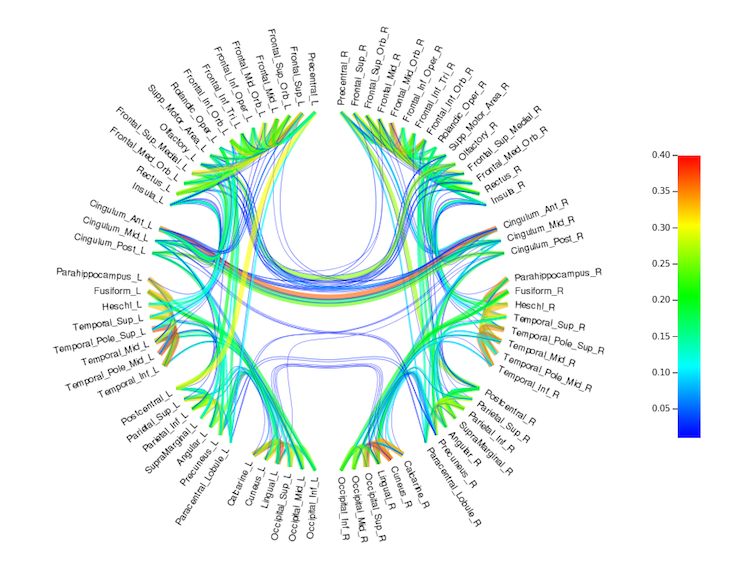
\includegraphics[width=8cm]{average_2y.png}}
\caption[Average brain connectome at 1 (a) and 2 (b) year old using the circle plotting ]{Average brain connectome at 1 (a) and 2 (b) year old using the circle plotting. Threshold : 0.01 - 0.4}
\label{fig:AverageBrainConnectome}
\end{figure} 

Figure \ref{fig:AverageBrainConnectome} is the circle plotting of the average brain connectome of our dataset. Figures \ref{fig:AverageBrainConnectomeBrainTemplate} shows the average brain connectome on brain template with the same threshold.

\begin{figure}
\centering 
\subfigure[]{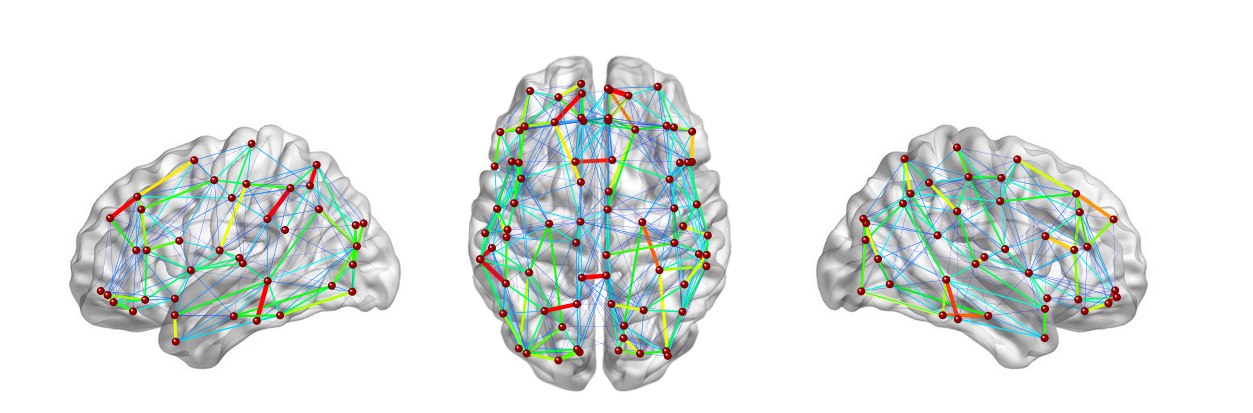
\includegraphics[width=8cm]{average_brainTemplate_1y.png}}
\subfigure[]{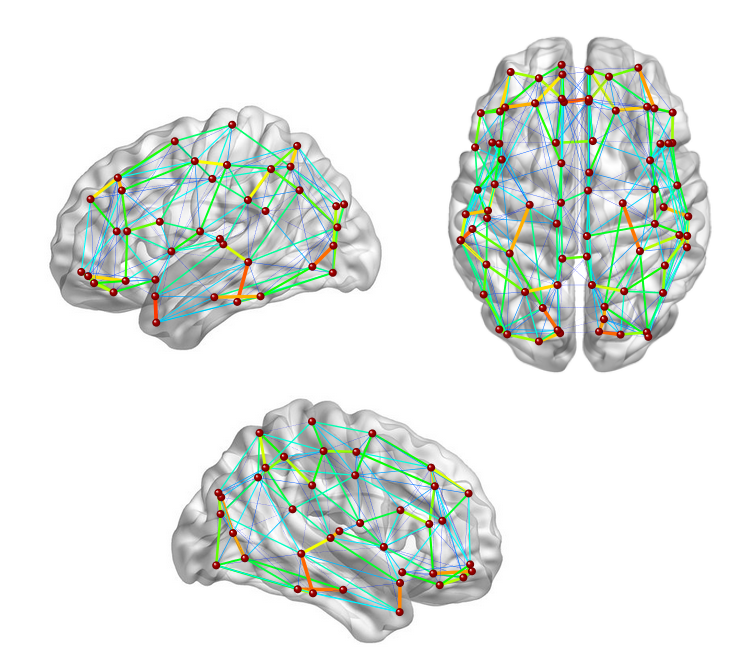
\includegraphics[width=8cm]{average_brainTemplate_2y.png}}
\caption[Average brain connectome at 1 (a) and 2 (b) year old on brain templates ]{Average brain connectome at 1 (a) and 2 (b) year old on brain templates. Threshold : 0.01 - 0.4}
\label{fig:AverageBrainConnectomeBrainTemplate}
\end{figure} 

First, we visualized that the shape of the connectivity is very similar at both ages. However, some links are missing in the brain connectome for 1 year old subjects. Moreover, the connectivity is lower for 1 year old children compared to 2 year children.


\subsection{Variability and deviation of the brain connectome}

We compute the unbiased sample variance  (equation \ref{equ:unbiasedSampleVariance}) to show the variability of the brain connectome in a dataset. 

\begin{equation}
	V_{i,j} = \frac{1}{n-1} \times \sum_{i=0, j=0}^n {(M_{i,j} - A_{i,j})^2}
	\label{equ:unbiasedSampleVariance}
\end{equation}

We also compute the standard deviation of this dataset at 1 and 2 year old (equation \ref{equ:standardDeviation}).

\begin{equation}
	D_{i,j} = \sqrt{V_{i,j}}
	\label{equ:standardDeviation}
\end{equation}

\begin{figure}
\centering 
\subfigure[]{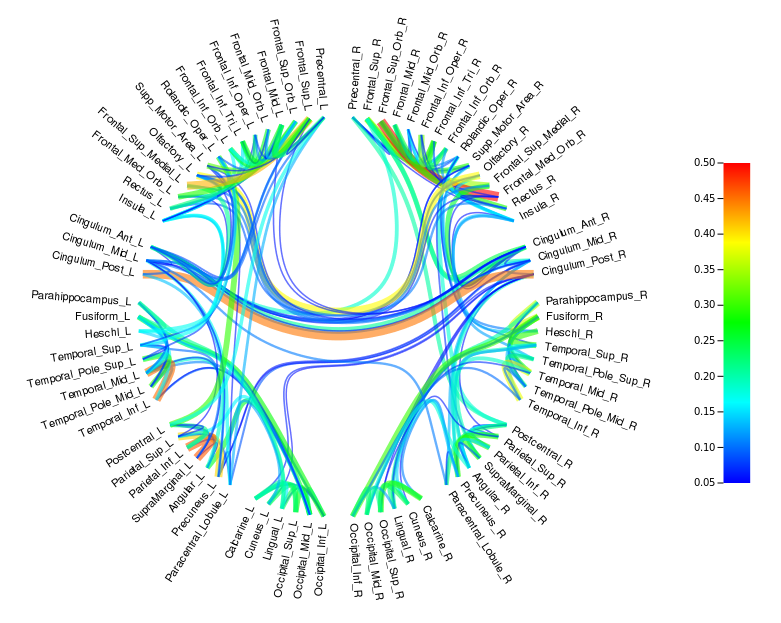
\includegraphics[width=8cm]{variance_1y.png}}
\subfigure[]{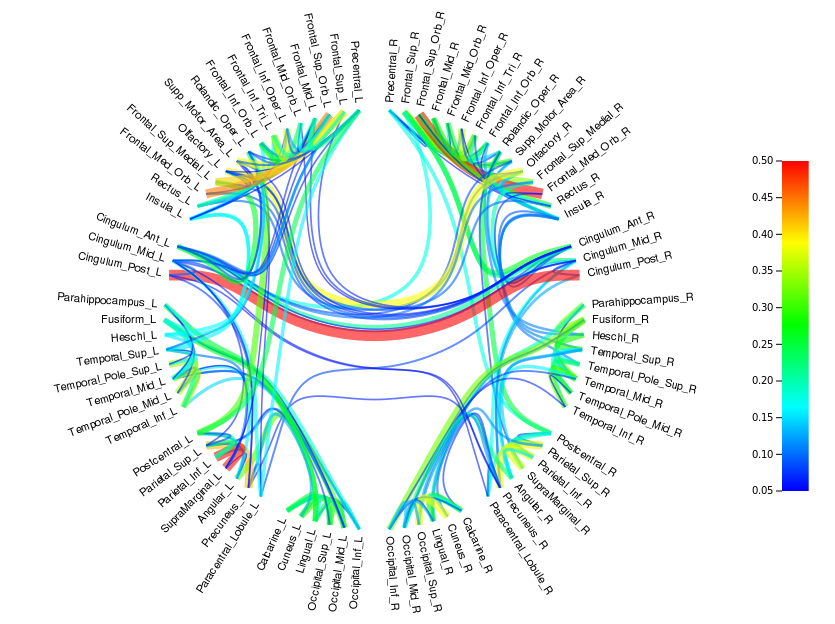
\includegraphics[width=8cm]{variance_2y.png}}
\caption[Variability of brain connectome at 1 (a) and 2 (a) year old using the circle plotting ]{Variability brain connectome at 1 and 2 year old using the circle plotting. Threshold : 0.05 - 0.5 }
\label{fig:VariabilityBrainConnectome}
\end{figure} 

\begin{figure}
\centering 
\subfigure[]{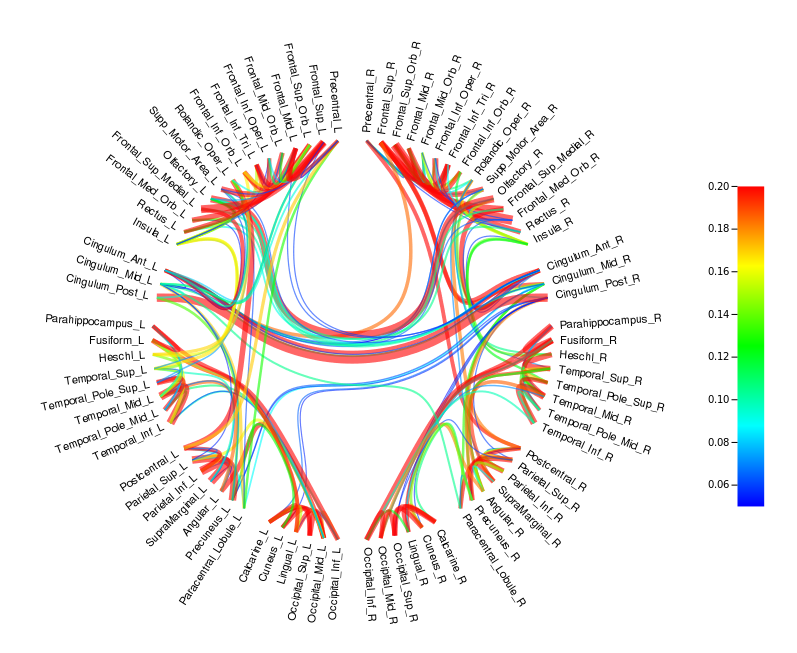
\includegraphics[width=8cm]{deviation_1y.png}}
\subfigure[]{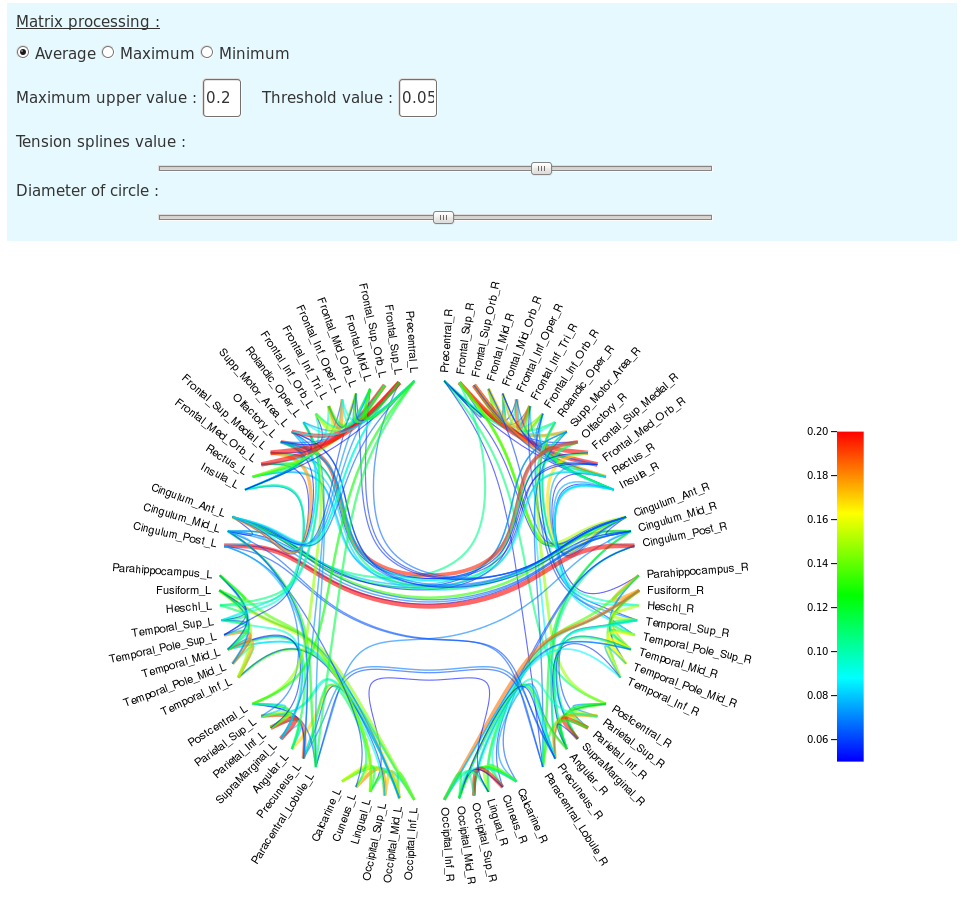
\includegraphics[width=8cm]{deviation_2y.png}}
\caption[Standard deviation of the brain connectome at 1 (a) and 2 (b) year old on brain templates ]{Standard deviation of the brain connectome at 1 (a) and 2 (b) year old on brain templates. Threshold : 0.05 - 0.5}
\label{fig:DeviationBrainConnectome}
\end{figure} 

The connectivity visualized in both figures is computed with the average value between the lower and upper triangles of the connectivity matrix.

Figure \ref{fig:VariabilityBrainConnectome} is showing the variability of the brain connectome at both ages. We threshold the plotting between 0.05 and 0.5 for a better visualization.
These results show a variability pretty constant between 1 and 2 year old, but a little bit higher at 2 years old.

Figure \ref{fig:DeviationBrainConnectome} shows the deviation if the brain connectome. 
We threshold the plotting between 0.05 and 0.2 for a better visualization. The circle plotting of the deviation of 1 year old infants shows a high deviation. The deviation of 2 year old infants dataset is much lower. This observation discloses brains connectome of 1 years infants are much different between them compare to the set of 2 years infants which are similar between them.

\section{CONCLUSIONS} 

We presented CIVILITY, Cloud based Interactive Visualization of Tractography Brain Connectome which is a  web tool in the cloud. The application is running a tractography pipeline and had visualization components. 

The tractography is using a probabilistic method (FSL tools) using surfaces as seeds. 
The visualization is showing the brain connectome by plotting the matrix in an interactive circle. 

CIVILITY offers to users the possibility to launch tractography really easily by only setting parameters and uploading files. 
The results of tractography are accessible from any station in the institution that which allows users to visualized results from any station connected to the institution. 

We have shown some statistics about infants' brains connectome and in the future, we expect thanks to this easy visualization to underline new aspect of brain development during childhood.








\acknowledgments

Thanks to Dr. Guilmore, UNC, for use of his dataset. Grants: UO1MH070890, U54HDO79124, RO1MH091351. 

%%%%%%%%%%%%%%%%%%%%%%%%%%%%%%%%%%%%%%%%%%%%%%%%%%%%%%%%%%%%%
%%%%% References %%%%%

\bibliography{report}   %>>>> bibliography data in report.bib
\bibliographystyle{spiebib}   %>>>> makes bibtex use spiebib.bst

\end{document} 
